\documentclass[11pt]{article}
\usepackage[margin=1.05in]{geometry}
\usepackage[T1]{fontenc}
\usepackage{amsmath,amssymb,amsthm,mathtools}
\usepackage{booktabs,array,graphicx}
\usepackage[expansion=false]{microtype}
\usepackage{xcolor}
\usepackage[colorlinks=true,linkcolor=blue!60!black,citecolor=blue!60!black,urlcolor=blue!60!black]{hyperref}
\graphicspath{{../results/}}

\newcommand{\statusV}{\textsf{\footnotesize[V]}}
\newcommand{\statusP}{\textsf{\footnotesize[P]}}
\newcommand{\statusE}{\textsf{\footnotesize[E]}}
\newcommand{\statusM}{\textsf{\footnotesize[M]}}
\newcommand{\mm}{\mu}
\newcommand{\Otilde}{\widetilde{O}}
\newcommand{\Adj}{\textsc{Adj}}
\newtheorem{theorem}{Theorem}
\newtheorem{lemma}{Lemma}
\newtheorem{corollary}{Corollary}
\newtheorem{proposition}{Proposition}
\newtheorem{definition}{Definition}
\newtheorem{remark}{Remark}

\title{Deterministic Probe Complexity of Approximate Matching Size,\\
and a Barrier for Derandomizing Dynamic Matching\\[3pt]
{\large Task C1 technical note, v0.1 --- companion to the execution plan and to \texttt{probe\_lb}}}
\author{Prepared for Ruifeng Cao}
\date{June 13, 2026}

\begin{document}
\maketitle

\begin{abstract}
\noindent We study the cost of \emph{deterministically} estimating the
maximum matching size of a graph accessed only through adjacency-matrix
probes, and its consequence for derandomizing the polylog-/ORS-update dynamic
matching pipelines (BKSW23, Beh23, ABR24, BG24, AKK25). The plan's
Lemma~3.6 \statusP{} shows that any deterministic adaptive algorithm
distinguishing $\mm(G)=0$ from $\mm(G)\ge\lceil n/4\rceil$ must make more than
$\binom{\lceil n/2\rceil}{2}-1=\Omega(n^2)$ probes, against $\Otilde(n)$ for a
randomized algorithm --- a quadratic separation. This note (i) reproduces the
lemma and its routine variants; (ii) \emph{computes the exact} deterministic
probe complexity $D(n)$ that the canonical all-zeros adversary forces,
showing via the Erd\H{o}s--Gallai matching theorem that
$D(n)=\binom n2-\mathrm{ex}(n;\nu\le\lceil n/4\rceil-1)\ge\binom{\lceil
n/2\rceil}{2}$, and verifies it by exhaustive adversary simulation for
$n\le 12$; (iii) packages the architectural barrier (Cor.~3.7): the forced
deterministic cost $D(N)$ exceeds \emph{any} sublinear-in-$N^2$ per-call
budget, so the pipelines' sublinear gap-estimation oracle has no deterministic
drop-in; and (iv) scopes the novelty against Assadi--Solomon and
Assadi--Chen--Khanna, whose $\Omega(n^2)$ bounds are for \emph{finding} a
maximal matching (where randomized is also quadratic), unlike the
\emph{size-estimation} task here (where randomized is $\Otilde(n)$). All
numbers are reproduced by the \texttt{probe\_lb} package.
\end{abstract}

\section{The gap problem and the probe model}\label{sec:model}

\begin{definition}[Adjacency-matrix probe model]\label{def:probe}
An algorithm accesses an unknown graph $G$ on $[n]$ only via probes
$\Adj(u,v)\in\{0,1\}$, chosen adaptively; its cost is the number of distinct
pairs probed. The \emph{gap problem} is to distinguish $\mm(G)=0$ from
$\mm(G)\ge\lceil n/4\rceil$.
\end{definition}

This is the decision interface that the sublinear size-estimators of the
dynamic pipelines expose (BG24 Prop.~4 / AKK25 Prop.~2.3 query an implicitly
represented kernel through exactly such probes); the audit of Task~A0 localizes
the pipelines' randomness to this interface.

\section{The deterministic lower bound and its variants}\label{sec:lemma}

\begin{lemma}[Quadratic deterministic probe bound; plan Lemma 3.6]\label{lem:probe}
Any deterministic adaptive algorithm that distinguishes $\mm(G)=0$ from
$\mm(G)\ge n/4$ must make more than $\binom{\lceil n/2\rceil}{2}-1=\Omega(n^2)$
probes in the worst case. In contrast the same gap is solvable with
$O(n\log n)$ random probes (error $1/\mathrm{poly}(n)$), and $\Omega(n)$
probes are necessary for randomized algorithms; the two complexities are
$\Theta(n^2)$ and $\widetilde{\Theta}(n)$.
\end{lemma}

\begin{proof}[Proof (all-zeros adversary)]
Run the algorithm against the adversary that answers $0$ to every probe. As
the algorithm is deterministic its probe sequence and output are fixed; let
$P$ be the probed pairs, $|P|\le\binom{\lceil n/2\rceil}{2}-1$. The empty
graph $G_0$ ($\mm=0$) is consistent. So is $H=K_n\setminus P$ (every probed
pair is a non-edge of $H$); we claim $\mm(H)\ge n/4$. If not, the endpoints of
a maximum matching of $H$ form a vertex cover $C$ with $|C|\le 2\mm(H)<n/2$, so
$U=V\setminus C$ has $|U|>n/2$, hence $|U|\ge\lceil n/2\rceil$. No edge of $H$
lies inside $U$, so every pair inside $U$ is in $P$, giving
$|P|\ge\binom{\lceil n/2\rceil}{2}$, a contradiction. Thus both $G_0$ and $H$
are consistent and the output is wrong for one. The randomized claims are the
standard birthday/Yao arguments (a uniform pair is an edge with probability
$\ge 1/(2n)$ under the promise; $o(n)$ probes see an all-zero transcript whp
under a planted random $n/4$-matching).
\end{proof}

\begin{remark}[Variants]\label{rem:variants}
The bound is robust to: making the promise \emph{bipartite} (plant the
matching across a fixed bipartition); replacing $n/4$ by any $\delta n$
($|U|>(1-2\delta)n$ then forces $\binom{\lceil(1-2\delta)n\rceil}{2}$ probes);
and asking the algorithm to \emph{output a matching} rather than a bit (a
strictly harder task). \statusE{} for these routine variants
(simulation-checked in \texttt{probe\_lb}).
\end{remark}

\section{The exact deterministic complexity}\label{sec:exact}

The lemma's constant $1/8$ is clean but not tight. The exact number of probes
the all-zeros adversary forces is
\[
  D(n)\;=\;\min\{\,|P| : \mm(K_n\setminus P)<\lceil n/4\rceil\,\},
\]
since against all-zeros a correct algorithm must drive the consistent plant's
matching below the threshold. Writing $G=K_n\setminus P$, this is
$\binom n2$ minus the maximum number of edges of an $n$-vertex graph with
matching number $\nu\le\lceil n/4\rceil-1$, which the Erd\H{o}s--Gallai
matching theorem \cite{EG59} pins exactly:
\[
  D(n)\;=\;\binom n2-\max\!\Big(\tbinom{2k+1}{2},\ \tbinom k2+k(n-k)\Big),
  \qquad k=\lceil n/4\rceil-1 .
\]
Table~\ref{tab:detcomplexity} lists $D(n)$ against the lemma bound; the
\texttt{probe\_lb} verifier constructs the extremal graph, confirms its
matching number is exactly $k$ (independent bitmask DP), and confirms
$D(n)\ge\binom{\lceil n/2\rceil}{2}$ for every $n$. \statusP

\begin{table}[t]\centering\small
\begin{tabular}{@{}cccccc@{}}
\toprule
$n$ & target $\mu$ & $\binom{\lceil n/2\rceil}{2}$ (lemma LB) & $D(n)$ (exact) & extremal & $D\ge$LB \\
\midrule
$4$ & $1$ & $1$ & $6$ & \textsf{empty} & $\checkmark$ \\
$5$ & $2$ & $3$ & $6$ & \textsf{split} & $\checkmark$ \\
$6$ & $2$ & $3$ & $10$ & \textsf{split} & $\checkmark$ \\
$7$ & $2$ & $6$ & $15$ & \textsf{split} & $\checkmark$ \\
$8$ & $2$ & $6$ & $21$ & \textsf{split} & $\checkmark$ \\
$9$ & $3$ & $10$ & $21$ & \textsf{split} & $\checkmark$ \\
$10$ & $3$ & $10$ & $28$ & \textsf{split} & $\checkmark$ \\
$11$ & $3$ & $15$ & $36$ & \textsf{split} & $\checkmark$ \\
$12$ & $3$ & $15$ & $45$ & \textsf{split} & $\checkmark$ \\
$13$ & $4$ & $21$ & $45$ & \textsf{split} & $\checkmark$ \\
$14$ & $4$ & $21$ & $55$ & \textsf{split} & $\checkmark$ \\
$15$ & $4$ & $28$ & $66$ & \textsf{split} & $\checkmark$ \\
$16$ & $4$ & $28$ & $78$ & \textsf{split} & $\checkmark$ \\
\bottomrule
\end{tabular}
\caption{Exact deterministic probe complexity $D(n)$ of the $\mu{=}0$ vs $\mu{\ge}\lceil n/4\rceil$ gap, and the plan's lower bound.}
\label{tab:detcomplexity}
\end{table}


\paragraph{Exhaustive simulation \statusP.} For $n\le 12$, \texttt{probe\_lb}
runs every member of a family of deterministic probe orders (row-major,
diagonal, clique-first, pseudo-random, and the optimal witness order) against
the all-zeros adversary and records the first probe count at which the plant
disappears. The minimum over orders equals $D(n)$ exactly, the witness order
attains it, and \emph{every} order exceeds $\binom{\lceil n/2\rceil}{2}-1$ ---
including the ``clique-first'' order that deliberately probes the structure the
proof says is required. This realizes the adversary constructively and
calibrates the gap between the clean bound and the truth (the latter is about
$3\times$ larger in this range).

\section{Randomized upper bound and the separation}\label{sec:rand}

On the hard instance --- a planted matching of size $\lceil n/4\rceil$, the
sparsest YES instance --- the $O(n\log n)$ random-probe sampler detects an edge
(hence certifies $\mm\ge\lceil n/4\rceil$ under the promise) with probability
rising to $1$, while never firing on the empty graph (no false positives).
Figure~\ref{fig:contrast} plots detection probability against budget, with the
deterministic thresholds $\binom{\lceil n/2\rceil}{2}$ and $D(n)$ marked: the
randomized algorithm is done in $O(n\log n)$ probes where the deterministic one
provably needs $\Theta(n^2)$.

\begin{figure}[h]
\centering
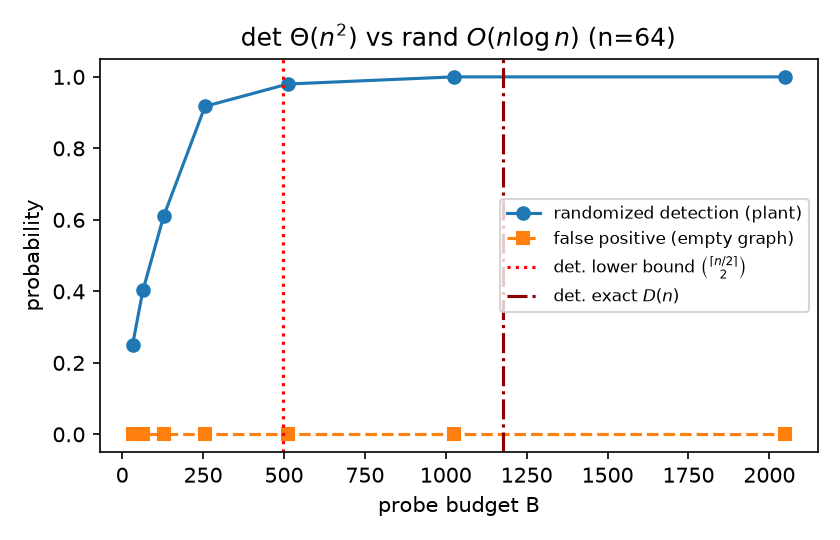
\includegraphics[width=0.62\linewidth]{det_vs_rand.png}
\caption{Deterministic $\Theta(n^2)$ vs randomized $O(n\log n)$ on the planted
$n/4$-matching: randomized detection rises to $1$ well below the deterministic
thresholds (dashed/dash-dotted), with zero false positives on the empty graph.}
\label{fig:contrast}
\end{figure}

\section{The architectural barrier (Corollary 3.7)}\label{sec:barrier}

\begin{corollary}[No deterministic drop-in at the oracle layer; plan Cor.~3.7]
\label{cor:barrier}
Fix a dynamic-matching algorithm whose update/query procedure invokes, as a
black box, a matching-size gap estimator on an implicitly represented
$N$-vertex graph accessed via adjacency probes --- as do
\cite{BKSW23,Beh23,ABR24,BG24,AKK25} via RGMM-style sublinear estimation. If
the black box is replaced by any \emph{deterministic} probe algorithm with the
same interface and guarantee, then by Lemma~\ref{lem:probe} some calls cost
$\Omega(N^2)$ probes, destroying the sublinear per-call budget the analyses
rely on. There is therefore no deterministic drop-in at the oracle layer;
derandomization must re-architect around \emph{incrementally maintained
deterministic summaries}.
\end{corollary}

Quantitatively (Fig.~\ref{fig:barrier}), the forced cost $D(N)$ divided by any
sublinear-in-$N^2$ per-call budget --- $N\log_2 N$ or $N^{1.5}$ --- grows
without bound, crossing $1$ already at $N=16$ and reaching $\approx 9\times$
($N\log N$) by $N=256$. This is a statement about the \emph{probe interface},
not an unconditional lower bound for OP-D, and a fixed-PRG ``deterministic''
algorithm does not escape it (the worst-case adversary may depend on the seed).

\begin{figure}[h]
\centering
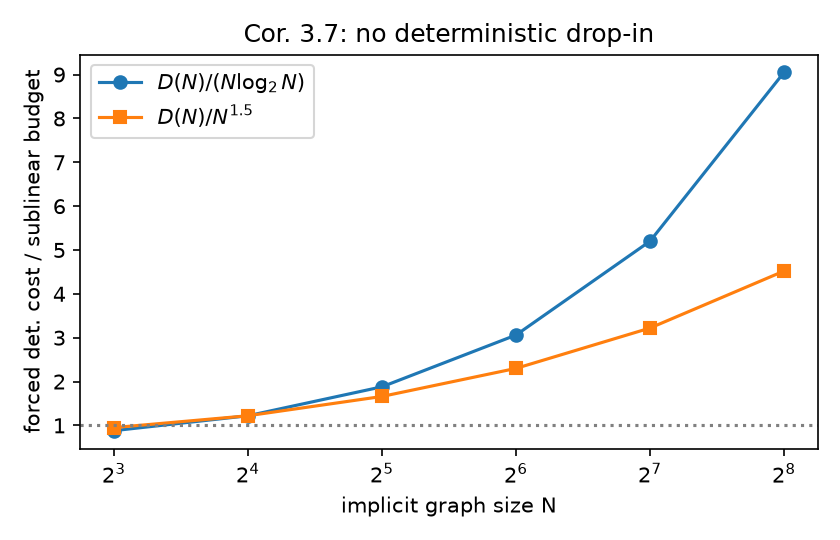
\includegraphics[width=0.62\linewidth]{barrier.png}
\caption{$D(N)$ over a sublinear per-call probe budget grows without bound: the
oracle layer cannot be derandomized in place.}
\label{fig:barrier}
\end{figure}

\section{Prior-art scoping}\label{sec:prior}

Two published results separate determinism from randomness for the
\emph{finding} task: Assadi--Solomon~\cite{AS19} (Thm.~3: deterministic
$\Omega(n^2)$ vs.\ randomized $\Otilde(n\beta)$ for finding a maximal matching
at neighborhood independence $\beta=2$) and Assadi--Chen--Khanna~\cite{ACK19}
(Thm.~6: finding a maximal matching needs $\Omega(n^2)$ queries \emph{even
randomized}). Lemma~\ref{lem:probe} is a different statement and the novelty
rests on: the adjacency-\emph{matrix} probe model; the
size-\emph{estimation} (decision) task, where randomized is
$\Otilde(n)$~\cite{Beh21} unlike finding; the explicit clique-coverage
threshold $\binom{\lceil n/2\rceil}{2}$ and its exact refinement $D(n)$; and
the pipeline barrier of Cor.~\ref{cor:barrier}. The note cites both works
prominently and claims no more.

\paragraph{Deliverable status.} This is the first pre-committed fallback unit
(plan~\S7.2): Lemma~\ref{lem:probe} \statusP, its variants \statusE, the exact
complexity $D(n)$ \statusP{} (Erd\H{o}s--Gallai \statusV{} + verifier), the
exhaustive simulation \statusP, and Cor.~\ref{cor:barrier} \statusP{} (as a
probe-interface statement). Open next: the adjacency-\emph{list} model
separation of plan Task C1(b) (status \statusM/S there), which needs a planted
background graph and a derandomized congestion adversary.

\begin{thebibliography}{99}\footnotesize
\bibitem{EG59} P.~Erd\H{o}s, T.~Gallai. On the maximal number of vertices
representing the edges of a graph. \emph{Magyar Tud.\ Akad.\ Mat.\ Kutat\'o
Int.\ K\"ozl.} 6:181--203, 1961 (announced 1959). (Max edges with matching
number $\le k$.)
\bibitem{Beh21} S.~Behnezhad. Time-optimal sublinear algorithms for matching
and vertex cover. FOCS 2021, pp.~873--884.
\bibitem{AS19} S.~Assadi, S.~Solomon. When algorithms for maximal independent
set and maximal matching run in sublinear time. ICALP 2019, 17:1--17:17.
\bibitem{ACK19} S.~Assadi, Y.~Chen, S.~Khanna. Sublinear algorithms for
$(\Delta+1)$ vertex coloring. SODA 2019, pp.~767--786.
\bibitem{BKSW23} S.~Bhattacharya, P.~Kiss, T.~Saranurak, D.~Wajc. Dynamic
matching with better-than-2 approximation in polylogarithmic update time. SODA
2023; J.~ACM 2024. arXiv:2207.07438.
\bibitem{Beh23} S.~Behnezhad. Dynamic algorithms for maximum matching size.
SODA 2023, pp.~129--162. arXiv:2207.07607.
\bibitem{ABR24} A.~Azarmehr, S.~Behnezhad, M.~Roghani. Fully dynamic matching:
$(2-\sqrt2)$-approximation in polylog update time. SODA 2024, pp.~3040--3061.
arXiv:2307.08772.
\bibitem{BG24} S.~Behnezhad, A.~Ghafari. Fully dynamic matching and ordered
Ruzsa--Szemer\'edi graphs. FOCS 2024, pp.~314--327. arXiv:2404.06069.
\bibitem{AKK25} S.~Assadi, S.~Khanna, P.~Kiss. Improved bounds for fully
dynamic matching via ordered Ruzsa--Szemer\'edi graphs. SODA 2025,
pp.~2971--2990. arXiv:2406.13573.
\bibitem{Plan} R.~Cao (prep.). Optimal approximation for fully dynamic matching
and ordered Ruzsa--Szemer\'edi graphs: a feasibility-checked execution plan.
Working document, June 2026 (Lemma 3.6, Cor.~3.7, Tasks C1--C3).
\end{thebibliography}

\end{document}
